\section{Методика и результаты тестирования}

Для обеспечения высокого качества и надежности нашего приложения для знакомств была разработана комплексная методика тестирования, включающая юнит-тестирование, интеграционное тестирование и нагрузочное тестирование.

\textbf{Юнит-тестирование:}
Каждый микросервис в системе подвергался тщательному юнит-тестированию. Юнит-тесты были разработаны для проверки корректности работы отдельных функций и методов в изоляции. Это позволило нам убедиться, что базовая логика каждого микросервиса функционирует правильно, и выявить возможные ошибки на ранних этапах разработки. Основные аспекты юнит-тестирования включали:
\begin{itemize}
    \item Проверка корректности реализации бизнес-логики.
    \item Валидация входных данных и проверка обработки исключений.
    \item Тестирование пограничных условий и различных сценариев использования.
\end{itemize}

\textbf{Интеграционное тестирование:}
После успешного прохождения юнит-тестов, микросервисы подвергались интеграционному тестированию. Интеграционные тесты проверяли корректность взаимодействия между различными микросервисами и компонентами системы. Особое внимание уделялось следующим аспектам:
\begin{itemize}
    \item Взаимодействие между микросервисами через gRPC.
    \item Корректность работы API Gateway при маршрутизации запросов.
    \item Проверка целостности данных при передаче между микросервисами.
\end{itemize}

\textbf{Нагрузочное тестирование:}
На финальном этапе разработки было проведено нагрузочное тестирование, целью которого являлась оценка производительности системы под высокими нагрузками. Мы использовали инструмент для симуляции большого количества одновременных пользователей (библиотека locust для python3) и запросов. Основные метрики, которые отслеживались во время нагрузочного тестирования, включали:
\begin{itemize}
    \item Время отклика микросервисов при различных уровнях нагрузки.
    \item Производительность базы данных PostgreSQL и ScyllaDB.
    \item Устойчивость системы к высоким нагрузкам и ее способность восстанавливаться после перегрузок.
\end{itemize}

\textbf{Результаты юнит и интеграционного тестирования:}
Результаты тестирования показали, что наше приложение удовлетворяет заданным требованиям по качеству и производительности:
\begin{itemize}
    \item Все микросервисы успешно прошли юнит-тесты, что подтвердило корректность их внутренней логики.
    \item Интеграционные тесты выявили и помогли устранить несколько проблем взаимодействия между микросервисами, обеспечив их бесшовную интеграцию.
\end{itemize}

\textbf{Результаты нагрузочного тестирования:}

В ходе нагрузочного тестирования были получены следующие результаты:

\begin{itemize}
    \item Для основных сценариев по созданию профиля, просмотру ленты и добавлению новых предложений для общения количество обработанных запросов в секунду составило примерно \textbf{5900 RPS}
    \item Для сценария с общением пользователей через мессенджер количество обработанных запросов в секунду составило примерно \textbf{984 RPS}
\end{itemize}

В \ref{stress_test_profiles} и \ref{stress_test_messenger} представлены графики, отражающие результаты нагрузочного тестирования для основных сценариев и мессенджера соответственно.
В целом, результаты нагрузочного тестирования показали, что наша система способна обрабатывать высокие нагрузки и обеспечивать стабильную производительность при различных сценариях использования.

\begin{landscape}
    \begin{figure}[!h]
        \centering
        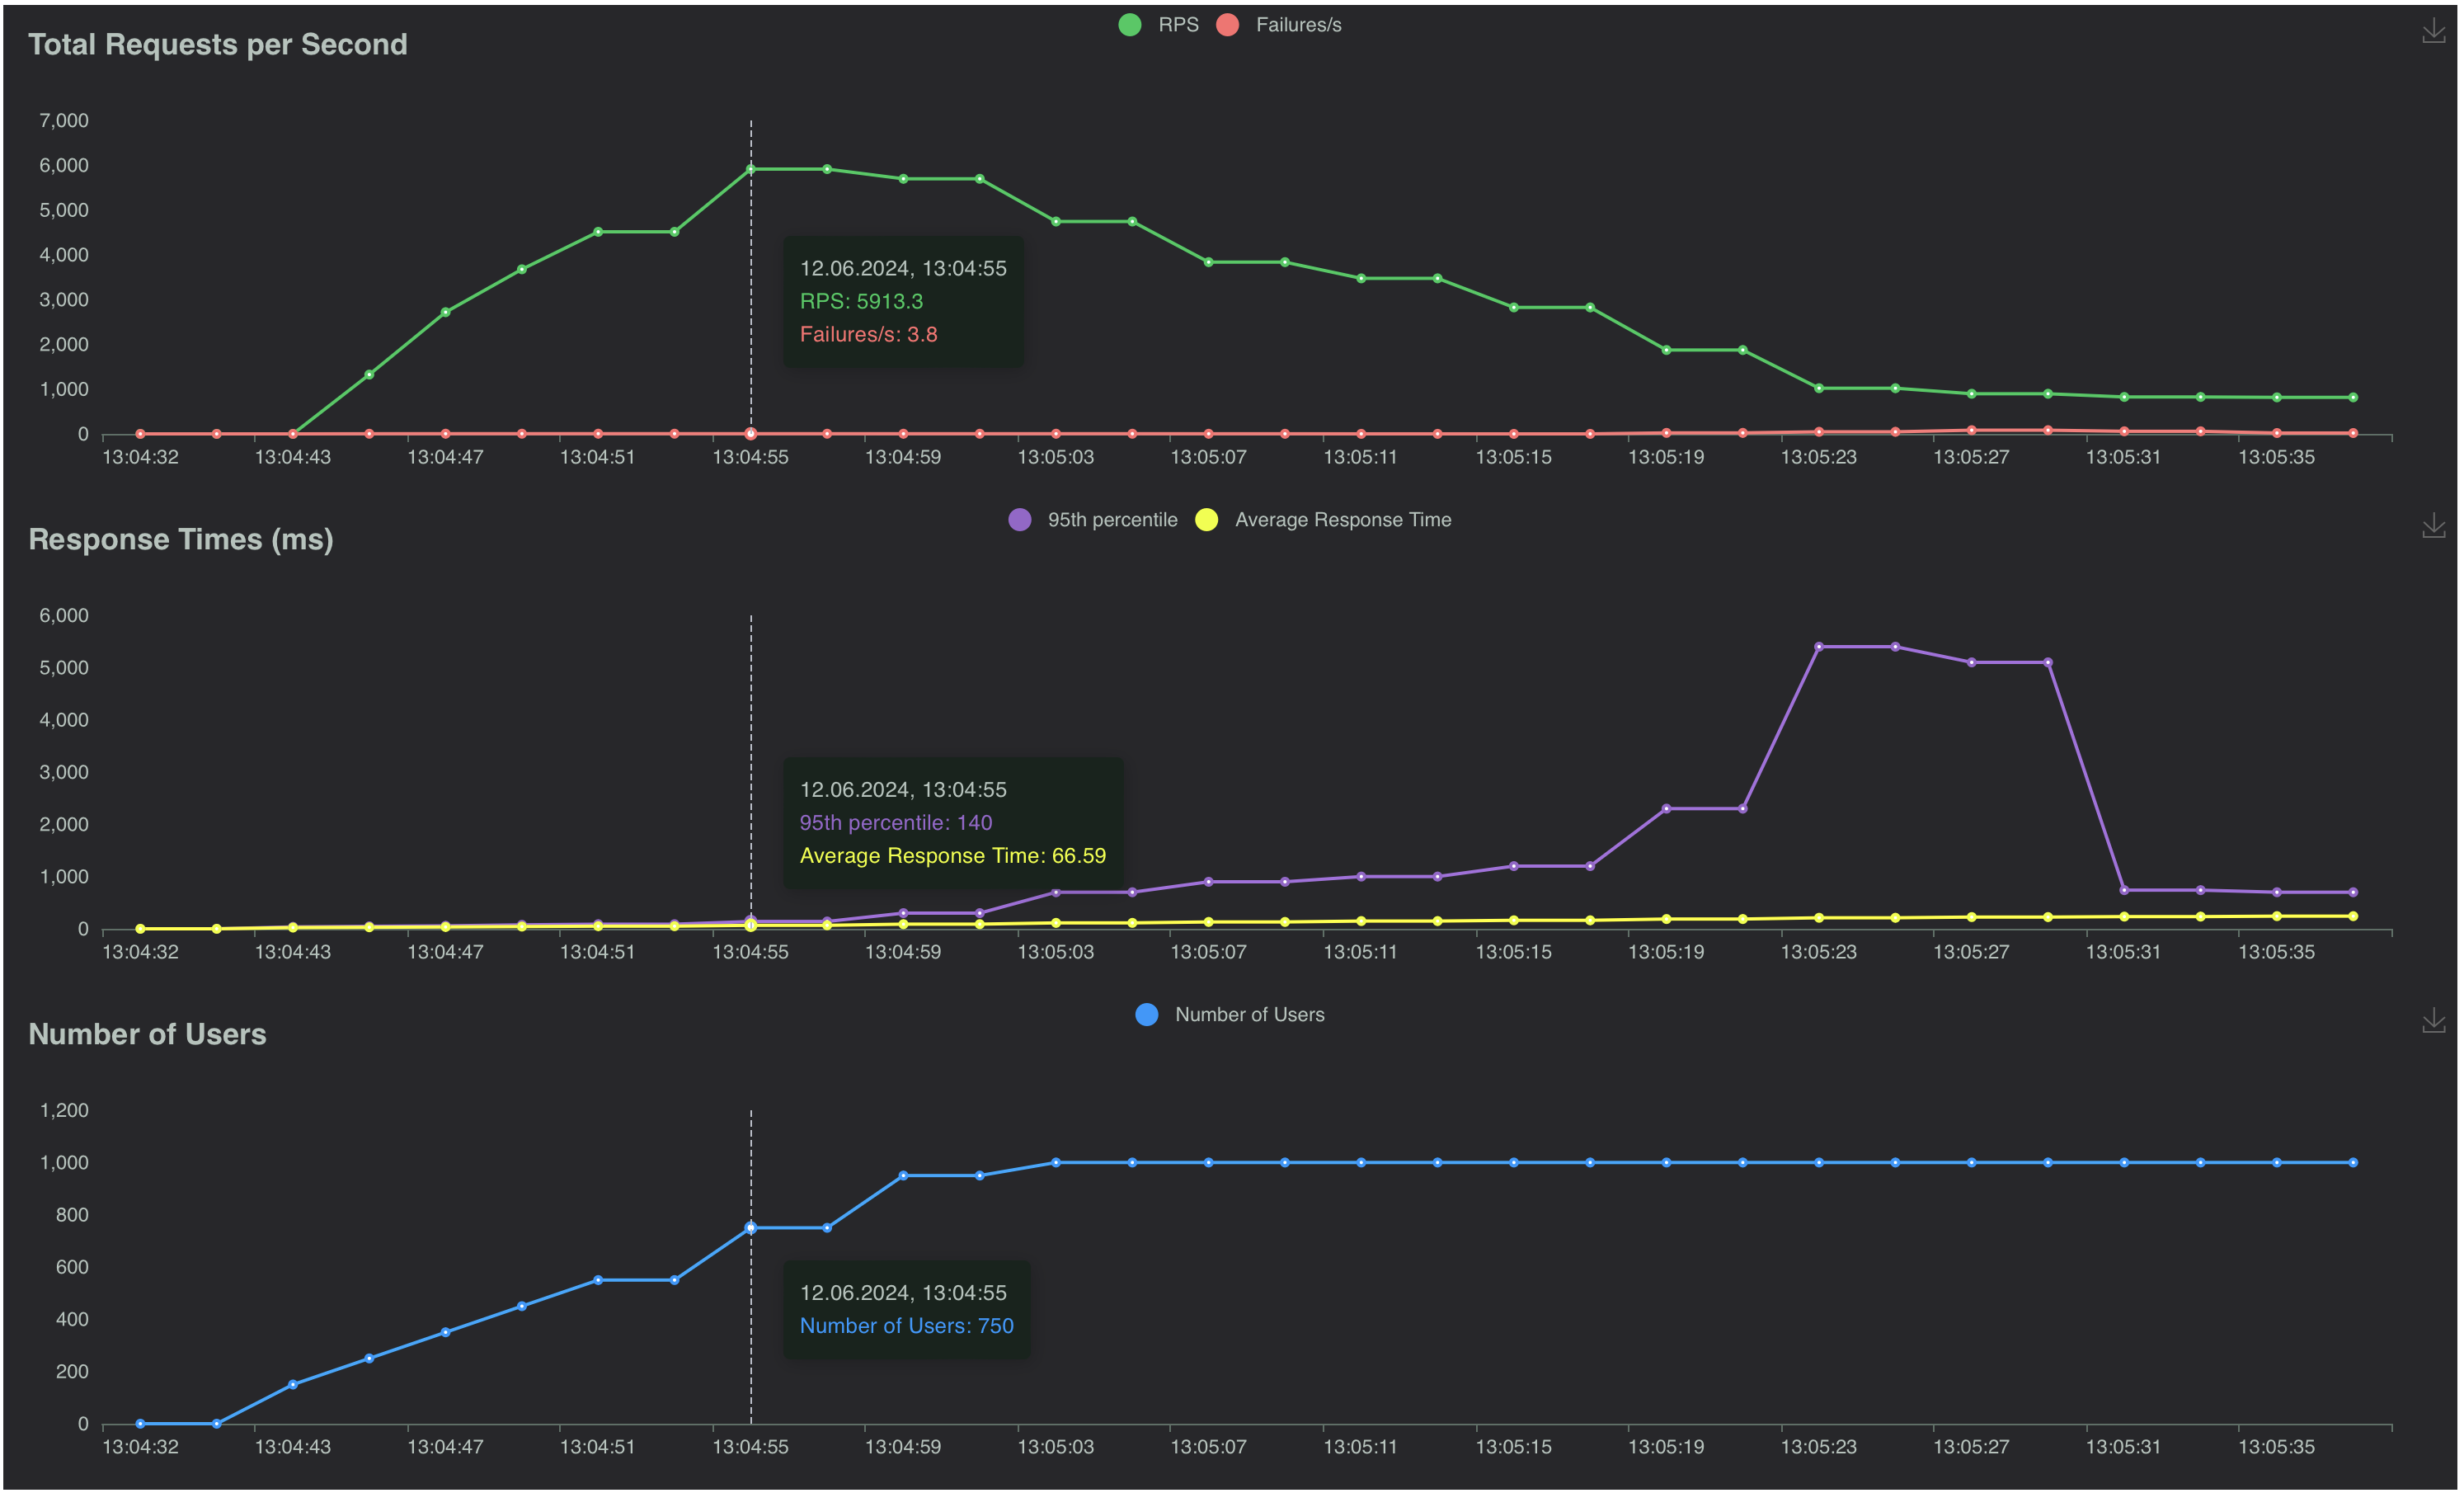
\includegraphics[height=0.8\textheight]{stress_test_results_profiles.png}
        \caption{Результаты нагрузочного тестирования для основных сценариев}
        \label{stress_test_profiles}
    \end{figure}
\end{landscape}

\begin{landscape}
    \begin{figure}[!h]
        \centering
        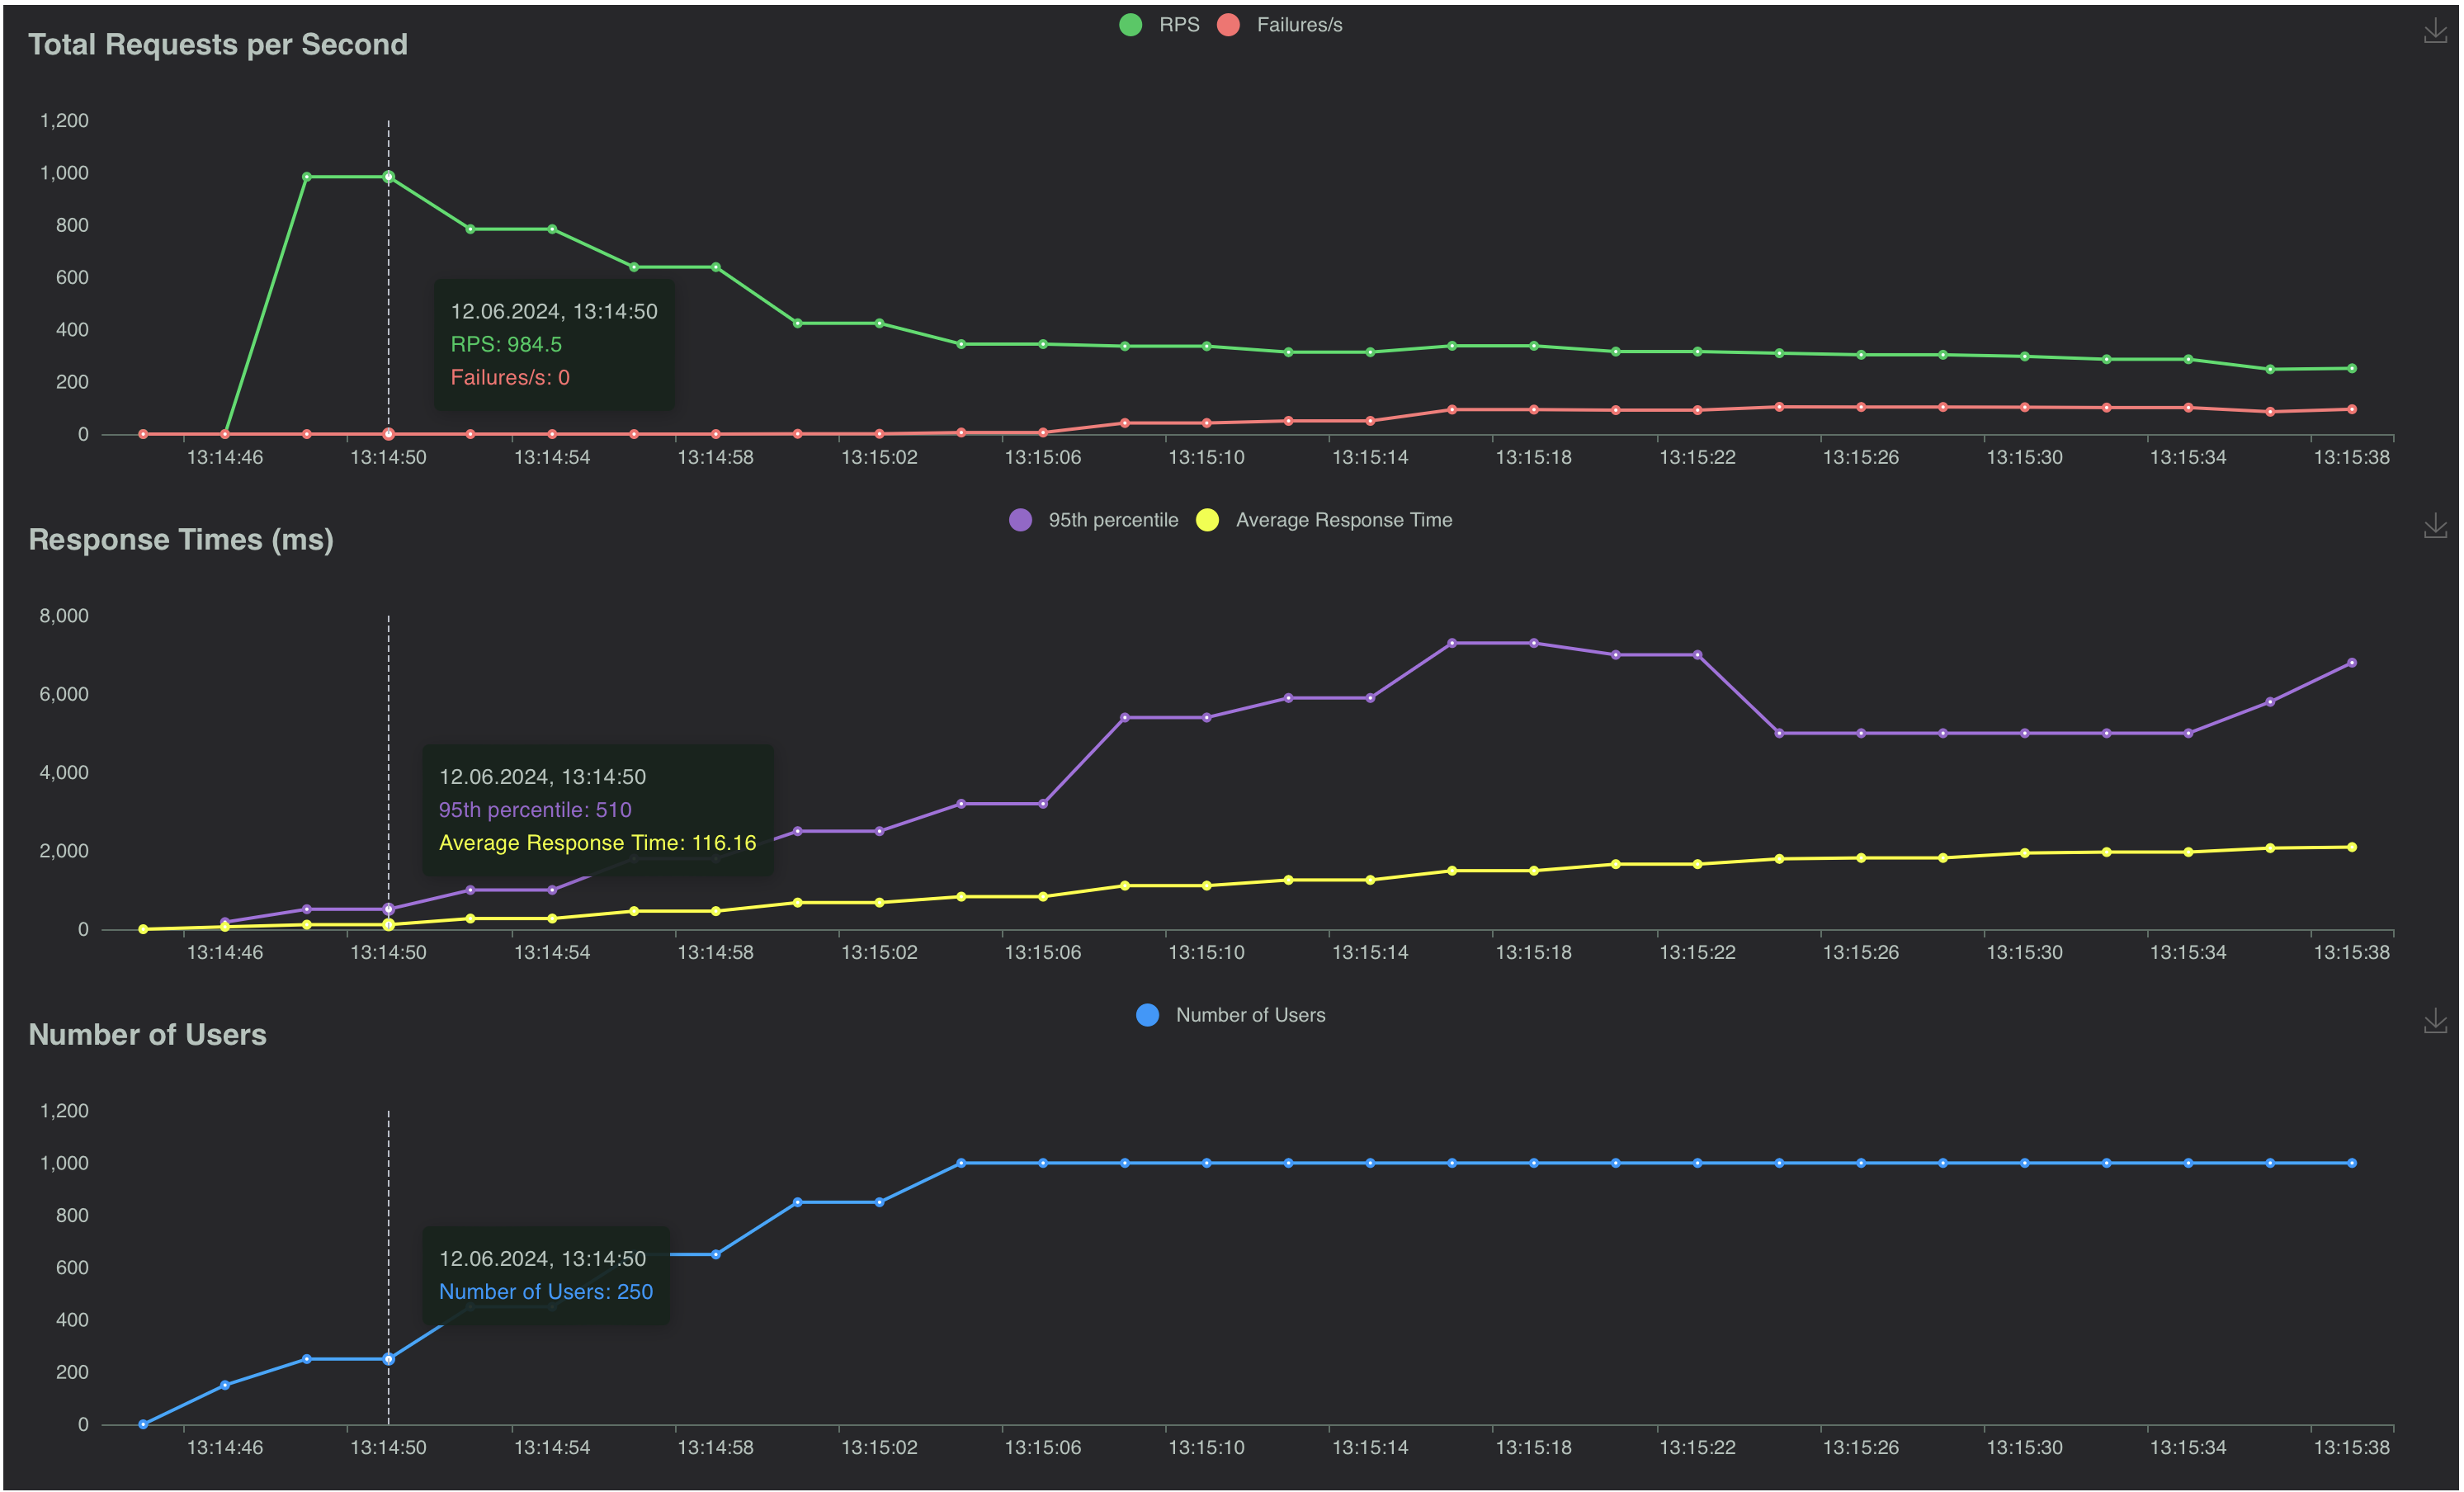
\includegraphics[height=0.8\textheight]{stress_test_results_messenger.png}
        \caption{Результаты нагрузочного тестирования для мессенджера}
        \label{stress_test_messenger}
    \end{figure}
\end{landscape}

